\documentclass[DIV=14,titlepage=false]{scrreprt}
\usepackage{parskip}
%%%%%%%%%%%%%%%%%%%%%%%%%%%%%%%%%%%%%%%%%%%%%%%%%%%%%%%%%%%%%%%%%%%%%%%%%%%%%%%
%                                Basic Packages                               %
%%%%%%%%%%%%%%%%%%%%%%%%%%%%%%%%%%%%%%%%%%%%%%%%%%%%%%%%%%%%%%%%%%%%%%%%%%%%%%%
% Gives us multiple colors.
\usepackage[usenames,dvipsnames,pdftex]{xcolor}
% Lets us style link colors.
\usepackage{hyperref}
% Lets us import images and graphics.
\usepackage{graphicx}
% Lets us use figures in floating environments.
\usepackage{float}
% Lets us create multiple columns.
\usepackage{multicol}
% Gives us better math syntax.
\usepackage{amsmath,amsfonts,mathtools,amsthm,amssymb}
% Lets us strikethrough text.
\usepackage{cancel}
% Lets us edit the caption of a figure.
\usepackage{caption}
% Lets us import pdf directly in our tex code.
\usepackage{pdfpages}
% Lets us do algorithm stuff.
\usepackage[ruled,vlined,linesnumbered]{algorithm2e}
% Gets rid of some errors.
\usepackage{scrhack}
\def\class{article}
\usepackage{geometry}
\geometry{margin=0.9in}
%%%%%%%%%%%%%%%%%%%%%%%%%%%%%%%%%%%%%%%%%%%%%%%%%%%%%%%%%%%%%%%%%%%%%%%%%%%%%%%
%                                Basic Settings                               %
%%%%%%%%%%%%%%%%%%%%%%%%%%%%%%%%%%%%%%%%%%%%%%%%%%%%%%%%%%%%%%%%%%%%%%%%%%%%%%%

%%%%%%%%%%%%%
%  Symbols  %
%%%%%%%%%%%%%

\let\implies\Rightarrow
\let\impliedby\Leftarrow
\let\iff\Leftrightarrow
\let\epsilon\varepsilon

%%%%%%%%%%%%
%  Tables  %
%%%%%%%%%%%%

\setlength{\tabcolsep}{5pt}
\renewcommand\arraystretch{1.5}

%%%%%%%%%%%%%%%%%%%%%%%
%  Center Title Page  %
%%%%%%%%%%%%%%%%%%%%%%%

\usepackage{titling}
\renewcommand\maketitlehooka{\null\mbox{}\vfill}
\renewcommand\maketitlehookd{\vfill\null}

%%%%%%%%%%%%%%%%%%%%%%%%%%%%%%%%%%%%%%%%%%%%%%%%%%%%%%%
%  Create a grey background in the middle of the PDF  %
%%%%%%%%%%%%%%%%%%%%%%%%%%%%%%%%%%%%%%%%%%%%%%%%%%%%%%%

\usepackage{eso-pic}
\newcommand\definegraybackground{
  \definecolor{reallylightgray}{HTML}{FAFAFA}
  \AddToShipoutPicture{
    \ifthenelse{\isodd{\thepage}}{
      \AtPageLowerLeft{
        \put(\LenToUnit{\dimexpr\paperwidth-222pt},0){
          \color{reallylightgray}\rule{222pt}{297mm}
        }
      }
    }
    {
      \AtPageLowerLeft{
        \color{reallylightgray}\rule{222pt}{297mm}
      }
    }
  }
}

%%%%%%%%%%%%%%%%%%%%%%%%
%  Modify Links Color  %
%%%%%%%%%%%%%%%%%%%%%%%%

\hypersetup{
  % Enable highlighting links.
  colorlinks,
  % Change the color of links to blue.
  linkcolor={black},
  % Change the color of citations to black.
  citecolor={black},
  % Change the color of url's to blue with some black.
  urlcolor=blue
}

%%%%%%%%%%%%%%%%%%
% Fix WrapFigure %
%%%%%%%%%%%%%%%%%%

\newcommand{\wrapfill}{\par\ifnum\value{WF@wrappedlines}>0
    \parskip=0pt
    \addtocounter{WF@wrappedlines}{-1}%
    \null\vspace{\arabic{WF@wrappedlines}\baselineskip}%
    \WFclear
\fi}

%%%%%%%%%%%%%%%%%
% Multi Columns %
%%%%%%%%%%%%%%%%%

\let\multicolmulticols\multicols
\let\endmulticolmulticols\endmulticols

\RenewDocumentEnvironment{multicols}{mO{}}
{%
  \ifnum#1=1
    #2%
  \else % More than 1 column
    \multicolmulticols{#1}[#2]
  \fi
}
{%
  \ifnum#1=1
\else % More than 1 column
  \endmulticolmulticols
\fi
}

\newlength{\thickarrayrulewidth}
\setlength{\thickarrayrulewidth}{5\arrayrulewidth}

%%%%%%%%%%%%%%%%%%%%
%  Import Figures  %
%%%%%%%%%%%%%%%%%%%%

\usepackage{import}
\pdfminorversion=7

% EXAMPLE:
% 1. \incfig{limit-graph}
% 2. \incfig[0.4]{limit-graph}
% Parameters:
% 1. The figure name. It should be located in figures/NAME.tex_pdf.
% 2. (Optional) The width of the figure. Example: 0.5, 0.35.
\newcommand\incfig[2][1]{%
  \def\svgwidth{#1\columnwidth}
  \import{./figures/}{#2.pdf_tex}
}

\begingroup\expandafter\expandafter\expandafter\endgroup
\expandafter\ifx\csname pdfsuppresswarningpagegroup\endcsname\relax
\else
  \pdfsuppresswarningpagegroup=1\relax
\fi

%%%%%%%%%%%%%
%  Correct  %
%%%%%%%%%%%%%

% EXAMPLE:
% 1. \correct{INCORRECT}{CORRECT}
% Parameters:
% 1. The incorrect statement.
% 2. The correct statement.
\definecolor{correct}{HTML}{009900}
\newcommand\correct[2]{{\color{red}{#1 }}\ensuremath{\to}{\color{correct}{ #2}}}



\newcommand{\R}{\mathbb{R}}
\newcommand{\Z}{\mathbb{Z}}
\newcommand{\E}{\mathbb{E}}
\newcommand{\B}{\ensuremath{\mathcal{B}}}
\newcommand{\X}{\ensuremath{\mathcal{X}}}
\newcommand{\Y}{\ensuremath{\mathcal{Y}}}
\newcommand{\mA}{\ensuremath{\mathbf{A}}}
\newcommand{\mB}{\ensuremath{\mathbf{B}}}
\newcommand{\mC}{\ensuremath{\mathbf{C}}}
\newcommand{\mD}{\ensuremath{\mathbf{D}}}
\newcommand{\mX}{\ensuremath{\mathbf{X}}}
\newcommand{\mY}{\ensuremath{\mathbf{Y}}}
\newcommand{\mx}{\ensuremath{\mathbf{x}}}
\newcommand{\my}{\ensuremath{\mathbf{y}}}
\newcommand{\mI}{\ensuremath{\mathbf{I}}}
\newcommand{\mi}{\ensuremath{\mathbf{\iota}}}
\newcommand{\mmu}{\ensuremath{\mathbf{\mu}}}
\newcommand{\mc}{\ensuremath{\mathbf{c}}}
\newcommand{\mSigma}{\ensuremath{\mathbf{\Sigma}}}
\newcommand{\mzero}{\ensuremath{\mathbf{0}}}
\newcommand{\independent}{\perp\!\!\!\!\perp} 
\setlength{\parindent}{0pt}
%%%%%%%%%%%%%%%%%%%%%%%%%%%%%%%%%%%%%%%%%%%%%%%%%%%%%%%%%%%%%%%%%%%%%%%%%%%%%%%
%                                 Environments                                %
%%%%%%%%%%%%%%%%%%%%%%%%%%%%%%%%%%%%%%%%%%%%%%%%%%%%%%%%%%%%%%%%%%%%%%%%%%%%%%%

\usepackage{varwidth}
\usepackage{thmtools}
\usepackage[most,many,breakable]{tcolorbox}

\tcbuselibrary{theorems,skins,hooks}
\usetikzlibrary{arrows,calc,shadows.blur}

%%%%%%%%%%%%%%%%%%%
%  Define Colors  %
%%%%%%%%%%%%%%%%%%%

\definecolor{myblue}{RGB}{45, 111, 177}
\definecolor{mygreen}{RGB}{56, 140, 70}
\definecolor{myred}{RGB}{199, 68, 64}
\definecolor{mypurple}{RGB}{197, 92, 212}

\definecolor{definition}{HTML}{228b22}
\definecolor{theorem}{HTML}{00007B}
\definecolor{example}{HTML}{2A7F7F}
\definecolor{definition}{HTML}{228b22}
\definecolor{prop}{HTML}{191971}
\definecolor{lemma}{HTML}{983b0f}
\definecolor{exercise}{HTML}{88D6D1}

\colorlet{definition}{mygreen!85!black}
\colorlet{claim}{mygreen!85!black}
\colorlet{corollary}{mypurple!85!black}
\colorlet{proof}{theorem}

%%%%%%%%%%%%%%%%%%%%%%
%  Helpful Commands  %
%%%%%%%%%%%%%%%%%%%%%%

% EXAMPLE:
% 1. \createnewtheoremstyle{thmdefinitionbox}{}{}
% 2. \createnewtheoremstyle{thmtheorembox}{}{}
% 3. \createnewtheoremstyle{thmproofbox}{qed=\qedsymbol}{
%       rightline=false, topline=false, bottomline=false
%    }
% Parameters:
% 1. Theorem name.
% 2. Any extra parameters to pass directly to declaretheoremstyle.
% 3. Any extra parameters to pass directly to mdframed.
\newcommand\createnewtheoremstyle[3]{
  \declaretheoremstyle[
  headfont=\bfseries\sffamily, bodyfont=\normalfont, #2,
  mdframed={
    #3,
  },
  ]{#1}
}

% EXAMPLE:
% 1. \createnewcoloredtheoremstyle{thmdefinitionbox}{definition}{}{}
% 2. \createnewcoloredtheoremstyle{thmexamplebox}{example}{}{
%       rightline=true, leftline=true, topline=true, bottomline=true
%     }
% 3. \createnewcoloredtheoremstyle{thmproofbox}{proof}{qed=\qedsymbol}{backgroundcolor=white}
% Parameters:
% 1. Theorem name.
% 2. Color of theorem.
% 3. Any extra parameters to pass directly to declaretheoremstyle.
% 4. Any extra parameters to pass directly to mdframed.
\newcommand\createnewcoloredtheoremstyle[4]{
  \declaretheoremstyle[
  headfont=\bfseries\sffamily\color{#2}, bodyfont=\normalfont, #3,
  mdframed={
    linewidth=2pt,
    rightline=false, leftline=true, topline=false, bottomline=false,
    linecolor=#2, backgroundcolor=#2!5, #4,
  },
  ]{#1}
}

%%%%%%%%%%%%%%%%%%%%%%%%%%%%%%%%%%%
%  Create the Environment Styles  %
%%%%%%%%%%%%%%%%%%%%%%%%%%%%%%%%%%%

\makeatletter
\@ifclasswith\class{nocolor}{
  % Environments without color.

  \createnewtheoremstyle{thmdefinitionbox}{}{}
  \createnewtheoremstyle{thmtheorembox}{}{}
  \createnewtheoremstyle{thmexamplebox}{}{}
  \createnewtheoremstyle{thmclaimbox}{}{}
  \createnewtheoremstyle{thmcorollarybox}{}{}
  \createnewtheoremstyle{thmpropbox}{}{}
  \createnewtheoremstyle{thmlemmabox}{}{}
  \createnewtheoremstyle{thmexercisebox}{}{}
  \createnewtheoremstyle{thmdefinitionbox}{}{}
  \createnewtheoremstyle{thmquestionbox}{}{}
  \createnewtheoremstyle{thmsolutionbox}{}{}

  \createnewtheoremstyle{thmproofbox}{qed=\qedsymbol}{}
  \createnewtheoremstyle{thmexplanationbox}{}{}
}{
  % Environments with color.

  \createnewcoloredtheoremstyle{thmdefinitionbox}{definition}{}{}
  \createnewcoloredtheoremstyle{thmtheorembox}{theorem}{}{}
  \createnewcoloredtheoremstyle{thmexamplebox}{example}{}{
    rightline=true, leftline=true, topline=true, bottomline=true
  }
  \createnewcoloredtheoremstyle{thmclaimbox}{claim}{}{}
  \createnewcoloredtheoremstyle{thmcorollarybox}{corollary}{}{}
  \createnewcoloredtheoremstyle{thmpropbox}{prop}{}{}
  \createnewcoloredtheoremstyle{thmlemmabox}{lemma}{}{}
  \createnewcoloredtheoremstyle{thmexercisebox}{exercise}{}{}

  \createnewcoloredtheoremstyle{thmproofbox}{proof}{qed=\qedsymbol}{backgroundcolor=white}
  \createnewcoloredtheoremstyle{thmexplanationbox}{example}{qed=\qedsymbol}{backgroundcolor=white}
}
\makeatother

%%%%%%%%%%%%%%%%%%%%%%%%%%%%%
%  Create the Environments  %
%%%%%%%%%%%%%%%%%%%%%%%%%%%%%

\declaretheorem[numberwithin=section, style=thmtheorembox,     name=Theorem]{theorem}
\declaretheorem[numbered=no,          style=thmexamplebox,     name=Example]{example}
\declaretheorem[numberwithin=section, style=thmclaimbox,       name=Claim]{claim}
\declaretheorem[numberwithin=section, style=thmcorollarybox,   name=Corollary]{corollary}
\declaretheorem[numberwithin=section, style=thmpropbox,        name=Proposition]{prop}
\declaretheorem[numberwithin=section, style=thmlemmabox,       name=Lemma]{lemma}
\declaretheorem[numberwithin=section, style=thmexercisebox,    name=Exercise]{exercise}
\declaretheorem[numbered=no,          style=thmproofbox,       name=Proof]{replacementproof}
\declaretheorem[numbered=no,          style=thmexplanationbox, name=Proof]{expl}

\makeatletter
\@ifclasswith\class{nocolor}{
  % Environments without color.

  \newtheorem*{note}{Note}

  \declaretheorem[numberwithin=section, style=thmdefinitionbox, name=Definition]{definition}
  \declaretheorem[numberwithin=section, style=thmquestionbox,   name=Question]{question}
  \declaretheorem[numberwithin=section, style=thmsolutionbox,   name=Solution]{solution}
}{
  % Environments with color.

  \newtcbtheorem[number within=section]{Definition}{Definition}{
    enhanced,
    before skip=2mm,
    after skip=2mm,
    colback=red!5,
    colframe=red!80!black,
    colbacktitle=red!75!black,
    boxrule=0.5mm,
    attach boxed title to top left={
      xshift=1cm,
      yshift*=1mm-\tcboxedtitleheight
    },
    varwidth boxed title*=-3cm,
    boxed title style={
      interior engine=empty,
      frame code={
        \path[fill=tcbcolback]
        ([yshift=-1mm,xshift=-1mm]frame.north west)
        arc[start angle=0,end angle=180,radius=1mm]
        ([yshift=-1mm,xshift=1mm]frame.north east)
        arc[start angle=180,end angle=0,radius=1mm];
        \path[left color=tcbcolback!60!black,right color=tcbcolback!60!black,
        middle color=tcbcolback!80!black]
        ([xshift=-2mm]frame.north west) -- ([xshift=2mm]frame.north east)
        [rounded corners=1mm]-- ([xshift=1mm,yshift=-1mm]frame.north east)
        -- (frame.south east) -- (frame.south west)
        -- ([xshift=-1mm,yshift=-1mm]frame.north west)
        [sharp corners]-- cycle;
      },
    },
    fonttitle=\bfseries,
    title={#2},
    #1
  }{def}

  \NewDocumentEnvironment{definition}{O{}O{}}
    {\begin{Definition}{#1}{#2}}{\end{Definition}}

  \newtcolorbox{note}[1][]{%
    enhanced jigsaw,
    colback=gray!20!white,%
    colframe=gray!80!black,
    size=small,
    boxrule=1pt,
    title=\textbf{Note:-},
    halign title=flush center,
    coltitle=black,
    breakable,
    drop shadow=black!50!white,
    attach boxed title to top left={xshift=1cm,yshift=-\tcboxedtitleheight/2,yshifttext=-\tcboxedtitleheight/2},
    minipage boxed title=1.5cm,
    boxed title style={%
      colback=white,
      size=fbox,
      boxrule=1pt,
      boxsep=2pt,
      underlay={%
        \coordinate (dotA) at ($(interior.west) + (-0.5pt,0)$);
        \coordinate (dotB) at ($(interior.east) + (0.5pt,0)$);
        \begin{scope}
          \clip (interior.north west) rectangle ([xshift=3ex]interior.east);
          \filldraw [white, blur shadow={shadow opacity=60, shadow yshift=-.75ex}, rounded corners=2pt] (interior.north west) rectangle (interior.south east);
        \end{scope}
        \begin{scope}[gray!80!black]
          \fill (dotA) circle (2pt);
          \fill (dotB) circle (2pt);
        \end{scope}
      },
    },
    #1,
  }

  \newtcbtheorem{Question}{Question}{enhanced,
    breakable,
    colback=white,
    colframe=myblue!80!black,
    attach boxed title to top left={yshift*=-\tcboxedtitleheight},
    fonttitle=\bfseries,
    title=\textbf{Question:-},
    boxed title size=title,
    boxed title style={%
      sharp corners,
      rounded corners=northwest,
      colback=tcbcolframe,
      boxrule=0pt,
    },
    underlay boxed title={%
      \path[fill=tcbcolframe] (title.south west)--(title.south east)
      to[out=0, in=180] ([xshift=5mm]title.east)--
      (title.center-|frame.east)
      [rounded corners=\kvtcb@arc] |-
      (frame.north) -| cycle;
    },
    #1
  }{def}

  \NewDocumentEnvironment{question}{O{}O{}}
  {\begin{Question}{#1}{#2}}{\end{Question}}

  \newtcolorbox{Solution}{enhanced,
    breakable,
    colback=white,
    colframe=mygreen!80!black,
    attach boxed title to top left={yshift*=-\tcboxedtitleheight},
    title=\textbf{Solution:-},
    boxed title size=title,
    boxed title style={%
      sharp corners,
      rounded corners=northwest,
      colback=tcbcolframe,
      boxrule=0pt,
    },
    underlay boxed title={%
      \path[fill=tcbcolframe] (title.south west)--(title.south east)
      to[out=0, in=180] ([xshift=5mm]title.east)--
      (title.center-|frame.east)
      [rounded corners=\kvtcb@arc] |-
      (frame.north) -| cycle;
    },
  }

  \NewDocumentEnvironment{solution}{O{}O{}}
  {\vspace{-10pt}\begin{Solution}{#1}{#2}}{\end{Solution}}
}
\makeatother

%%%%%%%%%%%%%%%%%%%%%%%%%%%%
%  Edit Proof Environment  %
%%%%%%%%%%%%%%%%%%%%%%%%%%%%

\renewenvironment{proof}[1][\proofname]{\vspace{-10pt}\begin{replacementproof}}{\end{replacementproof}}
\newenvironment{explanation}[1][\proofname]{\vspace{-10pt}\begin{expl}}{\end{expl}}

\theoremstyle{definition}

\newtheorem*{notation}{Notation}
\newtheorem*{previouslyseen}{As previously seen}
\newtheorem*{problem}{Problem}
\newtheorem*{observe}{Observe}
\newtheorem*{property}{Property}
\newtheorem*{intuition}{Intuition}



\title{%
R300 Econometrics}
\author{Metrics Enjoyers}
\date{Michaelmas Term, 2023-2024}

\setuptoc{toc}{leveldown}
\setcounter{chapter}{11}

\begin{document}
\pagenumbering{gobble}
\chapter{Probit Asymptotics. Testing Inequality Restrictions.}

\section{Asymptotics of Probit}

The conditional likelihood for the probit model is
\[L(\beta)=\prod_{i=1}^nf(y_i|x_i,\beta)\]
\[=\prod_{i=1}^nP(y_i=1|x_i,\beta)^{y_i}P(y_i=0|x_i,\beta)^{1-y_i}\]
\[=\prod_{i=1}^n\Phi(x_i'\beta)^{y_i}(1-\Phi(x_i'\beta))^{1-y_i}\]
and the conditional log-likelihood is
\[l(\beta)=\sum_{i=1}^ny_i\ln\Phi(x_i'\beta)+(1-y_i)\ln(1-\Phi(x_i'\beta))\]

Given \(x_i\), \(y_i\) we can find \(\hat(\beta_{ML})\) that maximises this function.

\vspace{5mm}
\begin{theorem} \textbf{The Probit Estimator}
\\ (i) \((\hat\beta_{prob})\xrightarrow{p}\beta_0\)
\\ (ii) \(\sqrt{n}(\hat\beta_{prob}-\beta_0)\xrightarrow{d}N(0,I_1^{-1})\) where,
\[I_1=E\left(\frac{\phi^2x_ix_i'}{\Phi(1-\Phi)}\right)\]
where \(\Phi=\Phi(x_i'\beta_0)\) and \(\phi=\frac{d}{dt}\Phi(t)\big|_{t=(x_i'\beta_0)}\)
\\ Under the following assumptions:
\begin{itemize}
    \item (Prob 0)\,\(\{y_i,x_i\}_{i=1}^n\) is an iid sequence with binary \(y_i\)
    \item (Prob 1)\,\(E(x_ix_i')\) is finite nonsingular
    \item (Prob 2)\,\(Pr(y_i=1|x_i)=\Phi(x_i'\beta)\)
\end{itemize}
\end{theorem}
\vspace{5mm}
\begin{proof}
The theorem follows from the fact that \(\hat{\beta}_{prob}\) is an MLE estimator. Indeed, the consistency statement is implied (as we have assumed correct distribution).

For the asymptotic normality, recall:
\[\sqrt{n}(\hat\theta_{ML}-\theta_0)\xrightarrow{d}N(0,n(I^{-1}(\theta_0)))\]
where \(\hat{\theta}_{ML}=\hat{\beta}_{prob} \text{ and } \theta_0=\beta_0\)

\[I(\beta)=Var\left(\frac{d}{d\beta}L(\beta)\right)\left(\stackrel{\beta=\beta_0}{=}E\left((\frac{d}{d\beta}L({\beta})\frac{d}{d\beta'}L({\beta}))\right)\right)\]
Since \(E(\frac{d}{d\beta}L(\beta))\big|_{\beta=\beta_0}=0\), as we have seen previously that this maximises the likelihood function.

\[\frac{dL(\beta)}{d\beta}=\sum_{i=1}^n\left(\frac{y_i}{\Phi(x_i'\beta)}\phi(x_i'\beta) x_i-\frac{(1-y_i)}{1-\Phi(x_i'\beta)}\phi(x_i'\beta)x_i\right)\]
\[=\sum_{i=1}^n\frac{y_i-\Phi(x_i'\beta)}{\Phi(x_i'\beta)(1-\Phi(x_i'\beta))}\phi(x_i'\beta)x_i\]

\[Var\frac{dL}{d\beta}=E(Var\frac{dL}{d\beta}|x_i)+Var(E(\frac{dL}{d\beta}|x_i))\]
\[Var(E(\frac{dL}{d\beta}|x_i))\big|_{\beta=\beta_0}=Var(0|x_i)=0\]

\[E(Var\frac{dL}{d\beta}|x_i)\big|_{\beta=\beta_0}=E Var\left(\sum_{i=1}^n\frac{y_i-\Phi(x_i'\beta)}{\Phi(x_i'\beta)(1-\Phi(x_i'\beta))}\phi(x_i'\beta)x_i|x_i\right)\]
Because iid,
\[=nEVar\left(\frac{y_i-\Phi(x_i'\beta)}{\Phi(x_i'\beta)(1-\Phi(x_i'\beta))}\phi(x_i'\beta)x_i|x_i\right)\]
since \(\Phi(x_i'\beta)\) is constant conditioning on \(x_i\):
\[=nEVar\left(\frac{y_i}{\Phi(x_i'\beta)(1-\Phi(x_i'\beta))}\phi(x_i'\beta)x_i|x_i\right)\]
\[=nE(\frac{\phi}{\Phi(1-\Phi)}x_i Var(y_i|x_i)\frac{\phi}{\Phi(1-\Phi)}x_i')\]

\(Var((y_i|x_i))\) is given by:
\[E(y_i^2|x_i)-E(y_i|x_i)^2\]
by Prob 2:
\[=(\Phi(1^2))-(\Phi(1))^2=\Phi-\Phi^2\]
Thus:
\[I(\beta_0)=nE\left(\frac{\phi^2x_ix_i'}{\Phi(1-\Phi)}\right)\]
\[I_1(\beta_0)=E\left(\frac{\phi^2x_ix_i'}{\Phi(1-\Phi)}\right)\]

\end{proof}

\subsection{Interpreting coefficients in Probit}
Unlike for linear regression, \(\beta=\beta_0\) cannot be interpreted as the marginal effect of \(x\) on \(y\). Here the coefficient measures the drect impact of regressors only on the (unobserved and scaled) underlying index. We are not typically interested in this slope but actually:
\begin{definition} \textbf{Probit Marginal Effects}
\[\frac{\partial Pr(y=1|x)}{\partial x_j}=\frac{\partial}{\partial x_j}(x'\beta)=\phi(x'\beta) \beta_j\]
here \(x_j\) refers to the \(j\)-th component of vector \(x\) as opposed to the \(j\)-th observation of this vector.
\\
Note that the effect depends not only on the value of \(x_j\) but also other variables.
\\
\underline{\smash{Marginal Effect at the Average:}}
\[\frac{\partial Pr(y=1|x)}{\partial x_j}\big|_{x=\bar{x}}=\phi(\bar{x}'\beta)\beta_j\]

Standard errors, use the delta method, where \(\theta=\beta\)
\[\frac{\partial Pr(y=1|x)}{\partial x_j}\big|_{x=\bar{x}}=\phi(\bar{x}'\beta)\beta_j=g(\beta)\]
Thus we have
\[\hat{Var}(\phi(\bar{x}'\beta)\beta_j)=\frac{1}{n}\frac{\partial g(\hat{\beta})}{\partial \beta'}\hat{I}_1^{-1}\frac{\partial g(\hat{\beta})}{\partial \beta}\]

\underline{\smash{Average Marginal Effect:}}
\[\frac{1}{n}\sum_{i=1}^n\frac{\partial Pr(y=1|x)}{\partial x_j}\big|_{x=x_i}=\frac{1}{n}\sum_{i=1}^n\phi(x_i'\beta)\beta_j\]
\end{definition}

\vspace{5mm}
\begin{note}
The ratios of the effects of two variables are equal to the ratio of their coefficients, and are therefore comparable for probit and logit models.
\[=\frac{\frac{\partial Pr(y=1|x)}{\partial x_j}}{\frac{\partial Pr(y=1|x)}{\partial x_k}}=\frac{\phi(x'\beta)\beta_j}{\phi(x'\beta)\beta_k}=\frac{\beta_j}{\beta_k}\]
Thus, while \(\hat{\beta}_j\) and \(\hat{\beta}_k\) are not directly interpretable as the absolute marginal effects, their ratio can be interpreted as the ratio of the marginal effects.
\end{note}

\section{Testing Inequality Constraints}
Instead of simply deleting or attempting to explain inconsistent signs of parameters in the estimating equation, we can statistically test whether or not the signs of the true values of these estimates are consistent with researcher beliefs.

Consider the stylised framework, of a normal regression model with two explanatory variables:

\[Y=\beta_1X1+\beta_2X2+\epsilon\]
where \(\epsilon|X_1,X_2\sim N(0,\sigma^2I_n)\) In addition, assume \(\sigma^2=1\) known and \(X_1,X_2\) orthonormal. That is, \(X'X=I_2\) where \(X=[X_1,X_2]\)

Suppose that we would like to test:
\[H_0:\beta_1\geq0 \text{ and } \beta_1\geq0 \text{ vs. }H_1:\beta_1<0 \text{ or } \beta_1<0\]

Let's derive the LR statistic. Recall that we assumed that it is known that \(\sigma^2=1\). Thus, the log-likelihood function is:
\(\log (max L(Y,\theta|X))\) without the restrictions:
\[=-\frac{n}{2}log(2\pi)-\frac{1}{2}(Y-X\hat{\beta}_{OLS})'(Y-X\hat{\beta}_{OLS})\]

\(\log (max L(Y,\theta|X))\) with the restrictions:
\[=-\frac{n}{2}log(2\pi)-\frac{1}{2}\operatorname*{min}_{b_1,b_2\geq0}(Y-Xb)'(Y-Xb)\]

Hence,
\[LR=\operatorname*{min}_{b_1,b_2\geq0}(Y-Xb)'(Y-Xb)-\frac{1}{2}(Y-X\hat{\beta}_{OLS})'(Y-X\hat{\beta}_{OLS})\]

Note that
\[(Y-Xb)'(Y-Xb)=Y'Y-2b'X'Y+b'X'Xb\]
\[=Y'Y-2b'X'(X\hat\beta_{OLS}+\hat\epsilon)+b'X'Xb\]
\[=Y'Y-2b'\hat\beta_{OLS}+b'b\]
and, similarly
\[(Y-X\hat\beta_{OLS})'(Y-X\hat\beta_{OLS})=Y'Y-\hat\beta_{OLS}'\hat\beta_{OLS}\]

Thus,
\[LR=\operatorname*{min}_{b_1,b_2\geq0}(\hat\beta_{OLS}-b)'(\hat\beta_{OLS}-b)\]

so that
\[LR=\begin{cases}0 & \text{ if }\hat\beta_{1,OLS}\geq0 \text{ and } \hat\beta_{2,OLS}\geq0
\\ \hat\beta_{1,OLS}^2 & \text{ if }\hat\beta_{1,OLS}<0 \text{ and } \hat\beta_{2,OLS}\geq0
\\ \hat\beta_{2,OLS}^2 & \text{ if }\hat\beta_{1,OLS}\geq0 \text{ and } \hat\beta_{2,OLS}<0
\\ \hat\beta_{1,OLS}^2+\hat\beta_{2,OLS}^2 & \text{ if }\hat\beta_{1,OLS}<0 \text{ and } \hat\beta_{2,OLS}<0
\end{cases}\]

Thus the LR statistic is the squared distance from \(\hat\beta_{OLS}\) to the positive quadrant in \(\R^2\):
\begin{center}
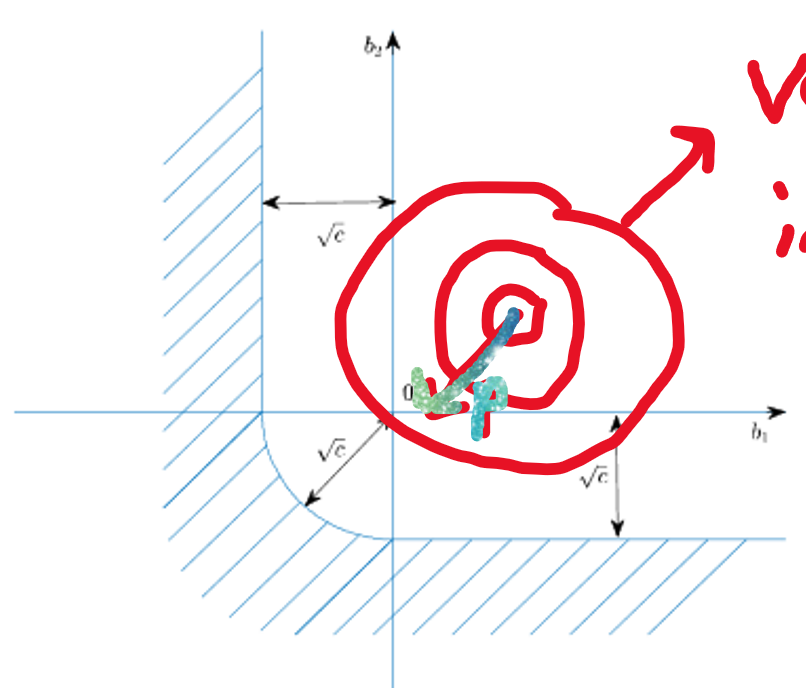
\includegraphics[width=0.5\textwidth]{./Images/LR test.png}
\end{center}

\underline{\smash{Finding c}}:
\\ If \(\beta_{OLS}\) ends up in the striped region (\(\Omega\)), LR test rejects. For the test with 5\% significance level, we need to choose the critical value \(c\) so that
\[\operatorname*{max}_{\beta_1,\beta_2\geq0}Pr(LR>c)=0.05\]

We can think of \(Pr(LR>c)|\beta=\beta_0\) as the volume of the probability density of \(\hat\beta_{OLS}\) that lies inside the critical region \(\Omega\).

Recall that \(\hat\beta_{OLS}|X\sim N(\beta_0,\sigma^2(X'X)^{-1})\)
In this special case:
\[\hat\beta_{OLS}|X\sim N(\beta_0,I_2)\]

Thus with this geometric interpretation
\[Pr(LR>c)=\int_{\Omega}\frac{1}{2\pi}exp\{-\frac{(z-\beta)'(z-\beta)}{2}\}dz\]
\[=\int_{\Omega-\beta}\frac{1}{2\pi}exp\{-\frac{z'z}{2}\}dz\]
where \(\Omega-\beta\) a linear shift of \(\Omega\). For any \(\beta\) from the positive quadrant (consistent with \(H_0\)), \(\Omega-\beta\subseteq\Omega\), with equality only at \(\beta=0\).
Therefore
\[\operatorname*{max}_{\beta_1,\beta_2\geq0}Pr(LR>c)=Pr(LR>c)|_{\beta_1=0,\beta_2=0}\]
This corresponds to the 'worst case' null, i.e. the case where it is hardest to differentiate between the null and alternative hypotheses.

On the other hand, if \(\beta_1=\beta_2=0\), then \(\hat\beta_{OLS}\) is distributed as \(N(0,I_2)\), thus \(\hat\beta_{1,OLS}^2\sim\chi^2(1)\) and \(\hat\beta_{2,OLS}^2\sim\chi^2(1)\), and \(\hat\beta_{1,OLS}^2+\hat\beta_{2,OLS}^2\sim\chi^2(2)\)

Thus,
\[LR=\begin{cases}0 & \text{ with probability 1/4 }
    \\ \chi^2(1) & \text{ with probability 1/2 }
    \\ \chi^2(2) & \text{ with probability 1/4 }
\end{cases}\]

Thus \(c\) is the 0.95 quantile of the mixture of chi-squared distributions. This can be found numerically.

\[F_{LR}(x)= 1/4F_0(x)+1/2F_{\chi^2(1)}(x)+1/4F_{\chi^2(2)}(x)\]

\end{document}